% ======================= Appendices =======================
\renewcommand{\thefigure}{A.\arabic{figure}}
\setcounter{figure}{0}
\appendixchapter{APPENDIX A: Snapshots}
This appendix shows the main screens of the deployed ScamGuard application.
\begin{figure}[H]\centering\fbox{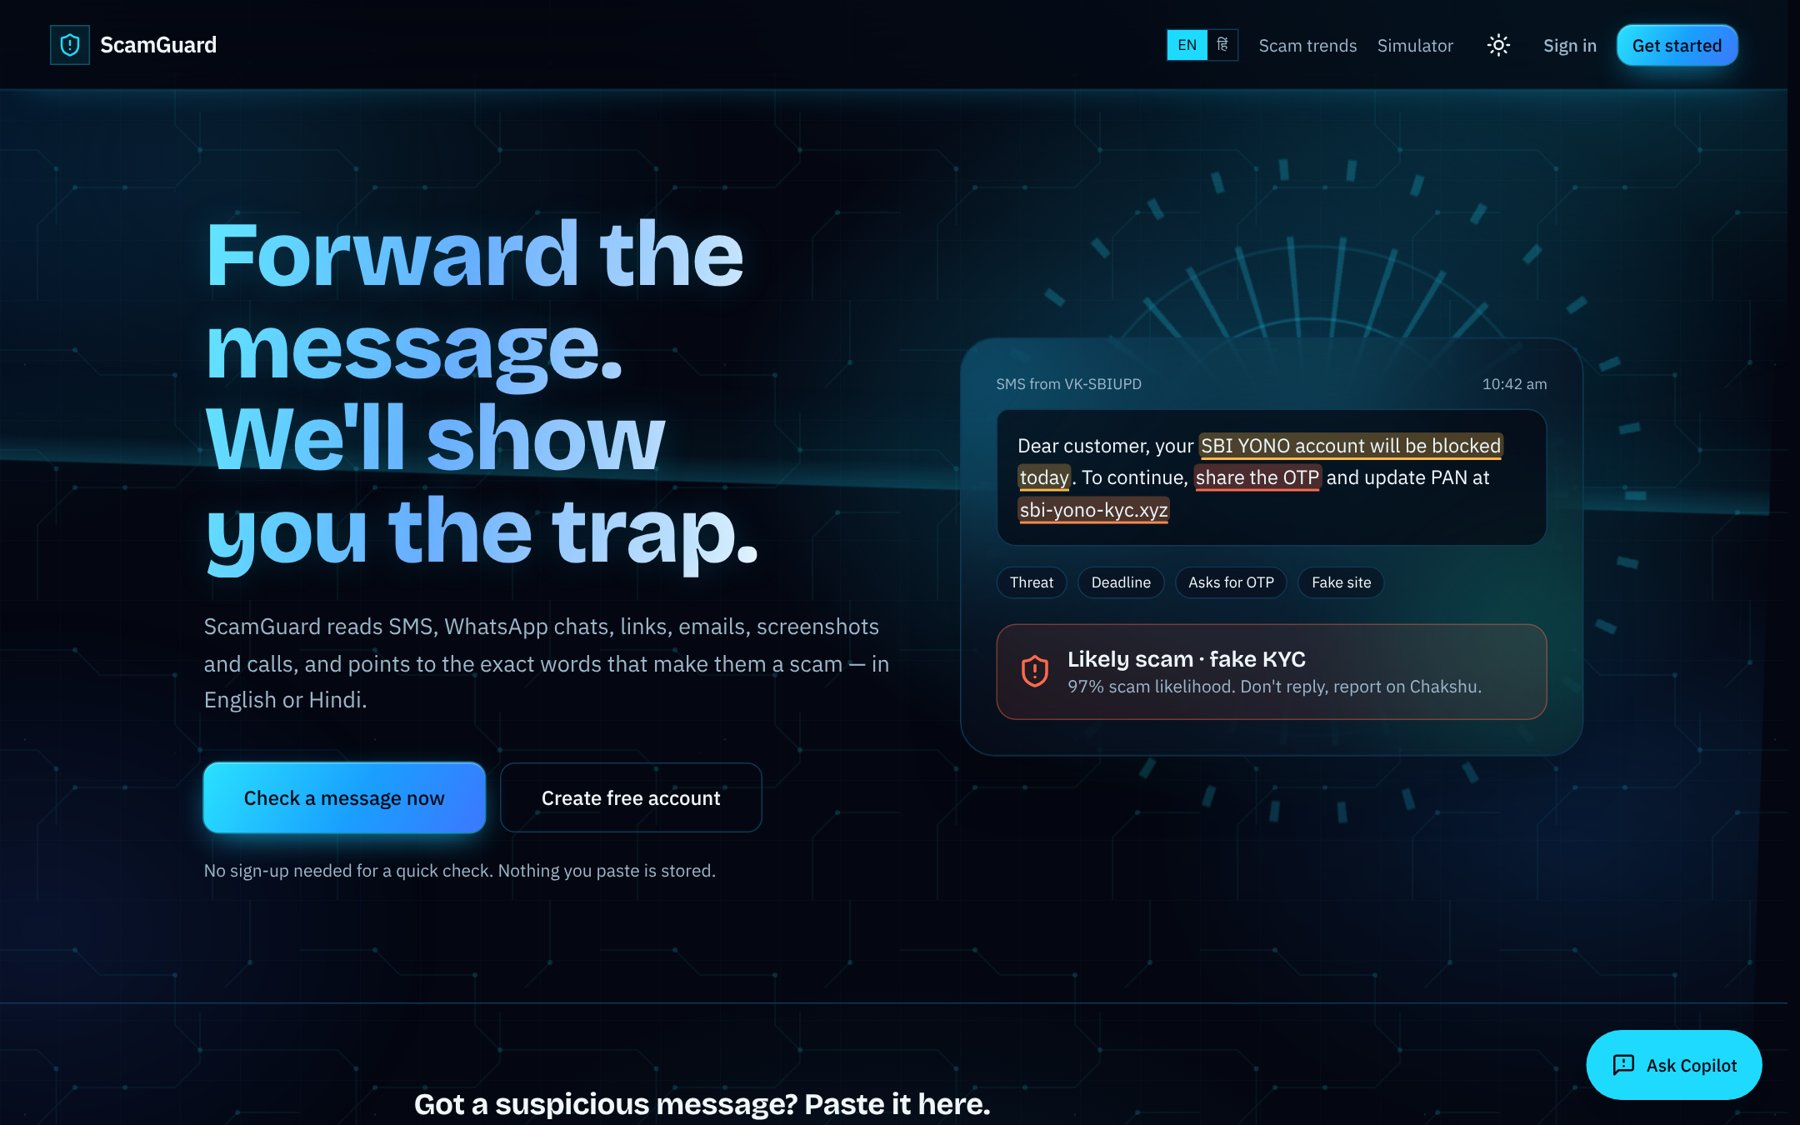
\includegraphics[width=0.80\linewidth,height=0.36\textheight,keepaspectratio]{shots/01_landing.jpg}}\caption{Home page with the quick check}\end{figure}
\begin{figure}[H]\centering\fbox{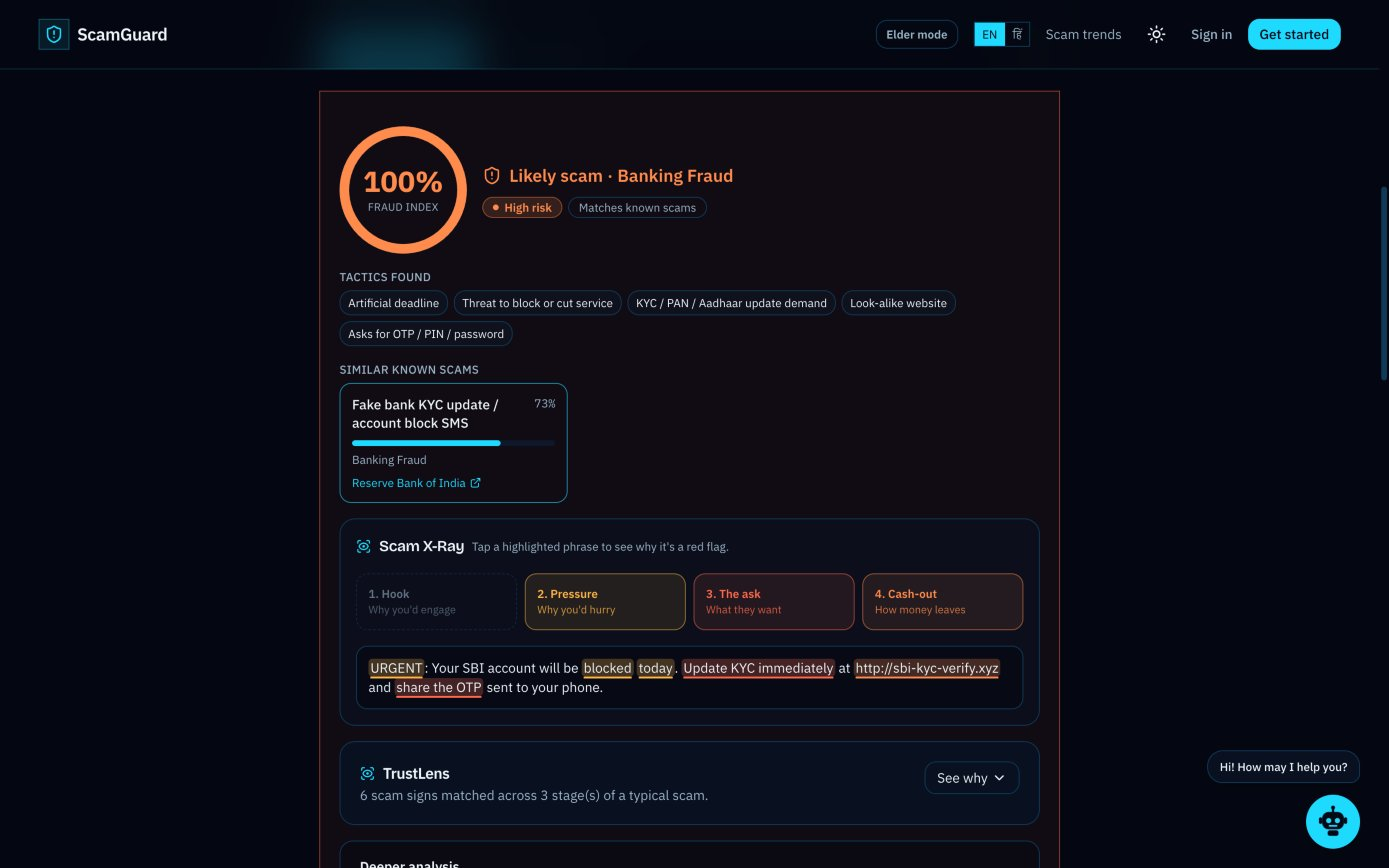
\includegraphics[width=0.80\linewidth,height=0.36\textheight,keepaspectratio]{shots/02_quick_scam.jpg}}\caption{Quick check of a fake KYC message: verdict, matched tactics, known pattern and Scam X-Ray}\end{figure}
\begin{figure}[H]\centering\fbox{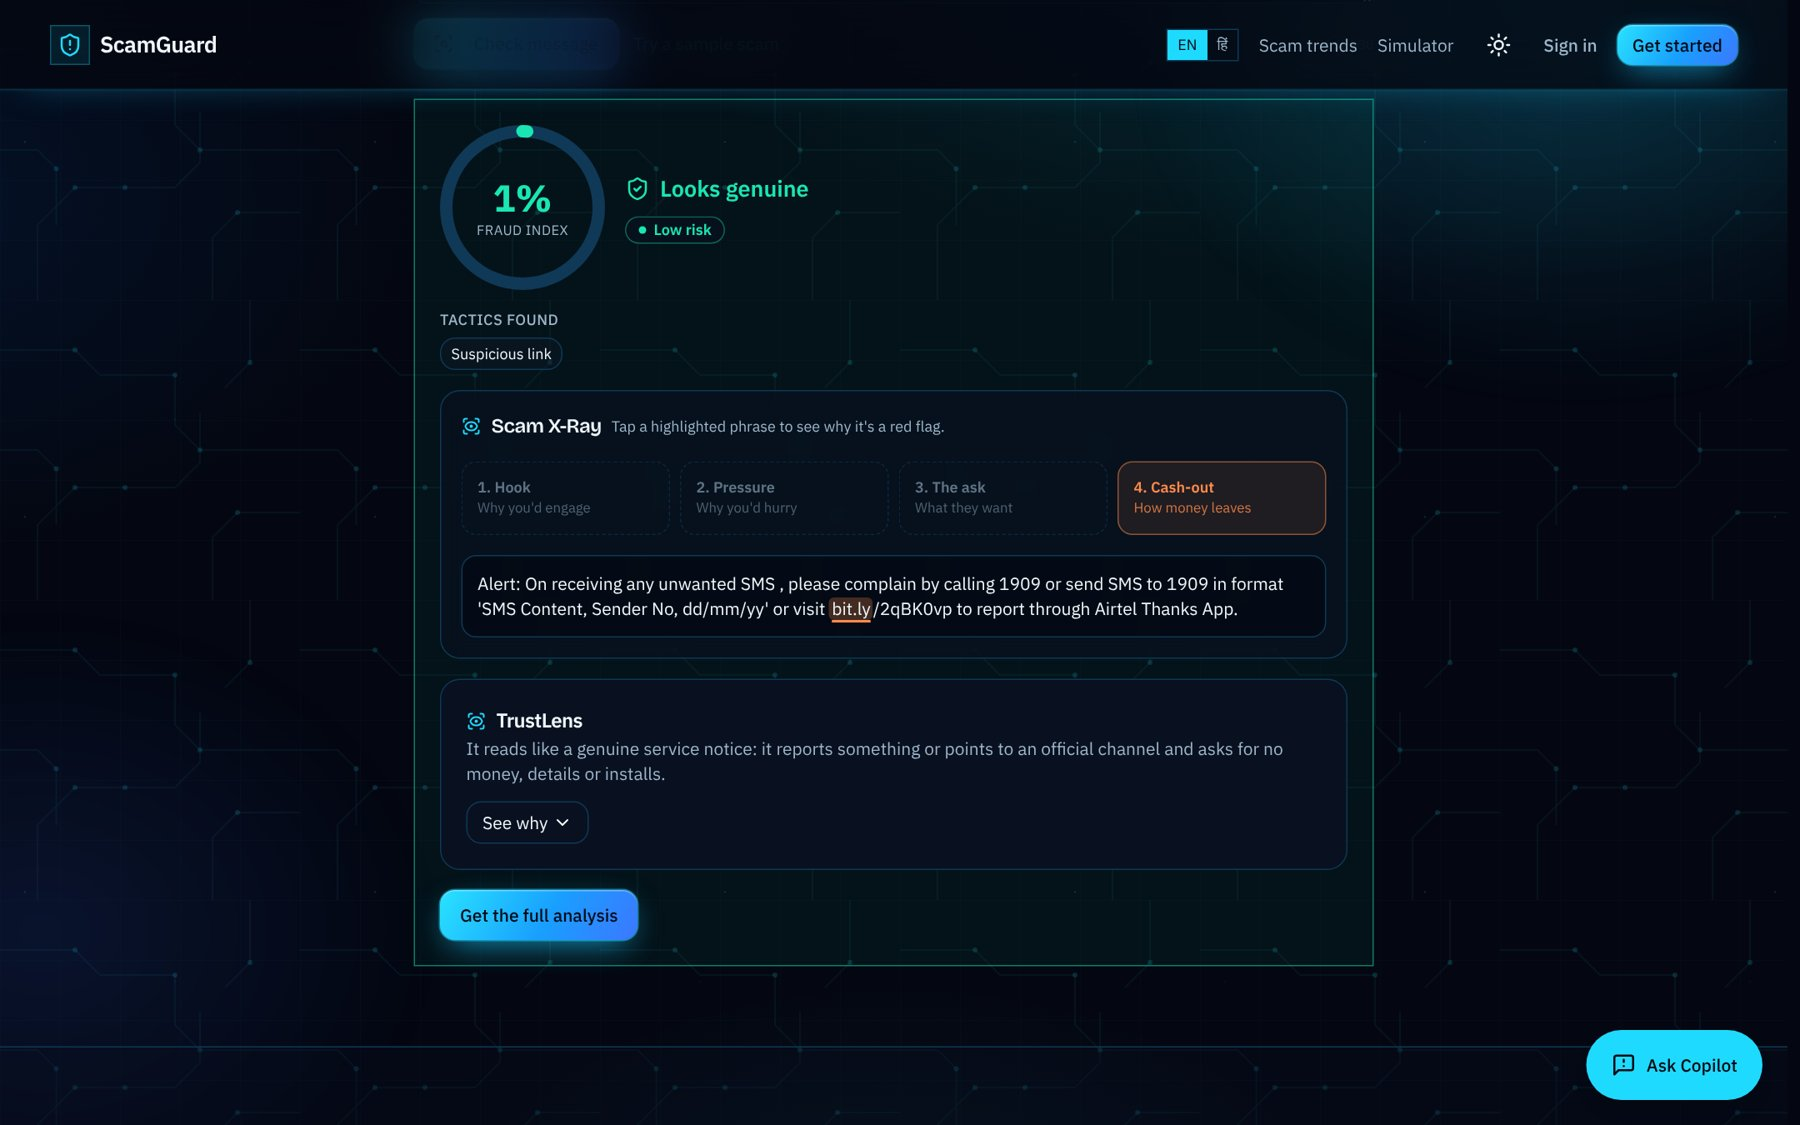
\includegraphics[width=0.80\linewidth,height=0.36\textheight,keepaspectratio]{shots/03_quick_genuine.jpg}}\caption{Quick check of a genuine operator notice about the 1909 helpline, marked as looking genuine with the TrustLens reason}\end{figure}
\begin{figure}[H]\centering\fbox{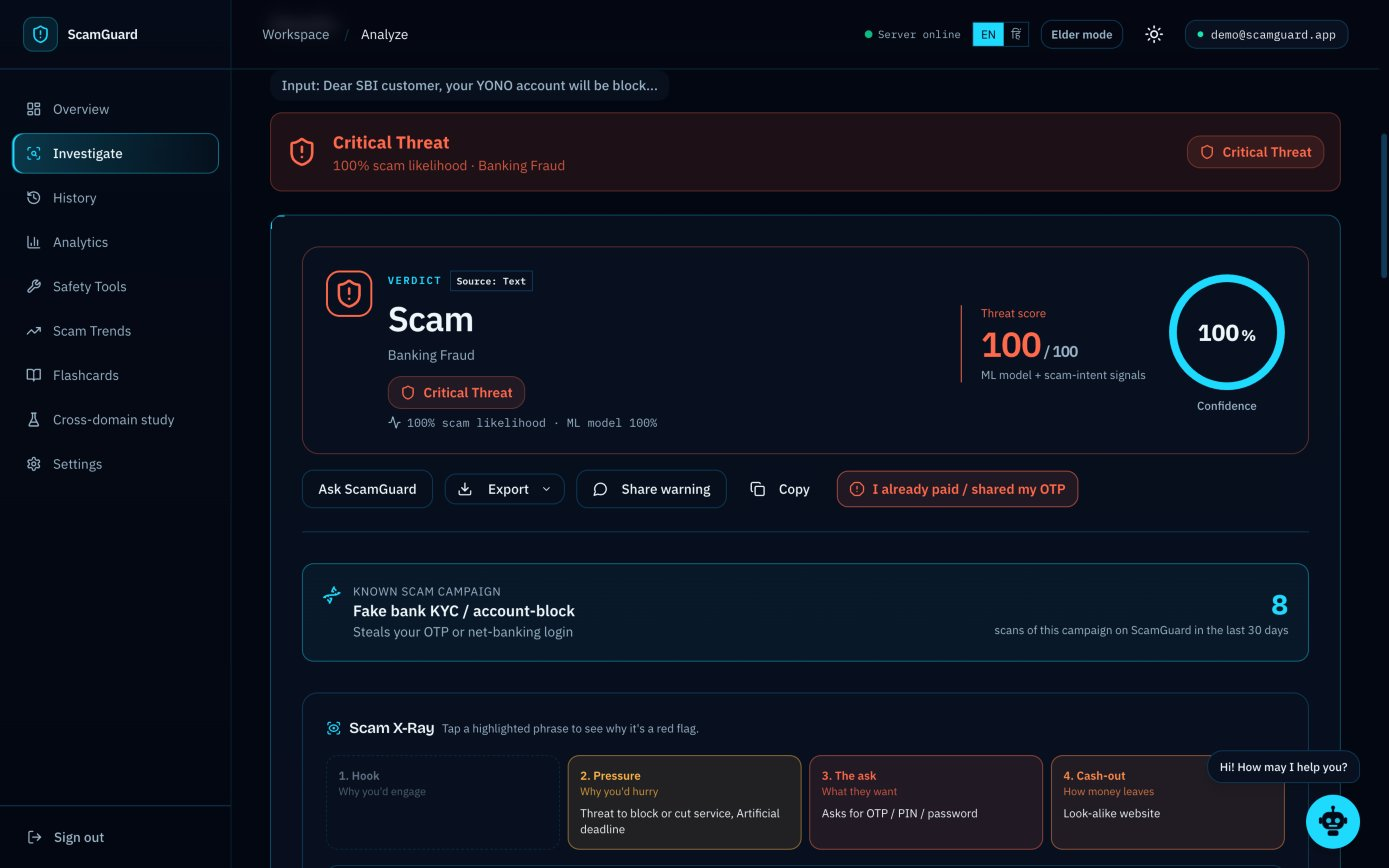
\includegraphics[width=0.80\linewidth,height=0.36\textheight,keepaspectratio]{shots/05_analyze_result.jpg}}\caption{Full analysis of a scam message for a signed-in user}\end{figure}
\begin{figure}[H]\centering\fbox{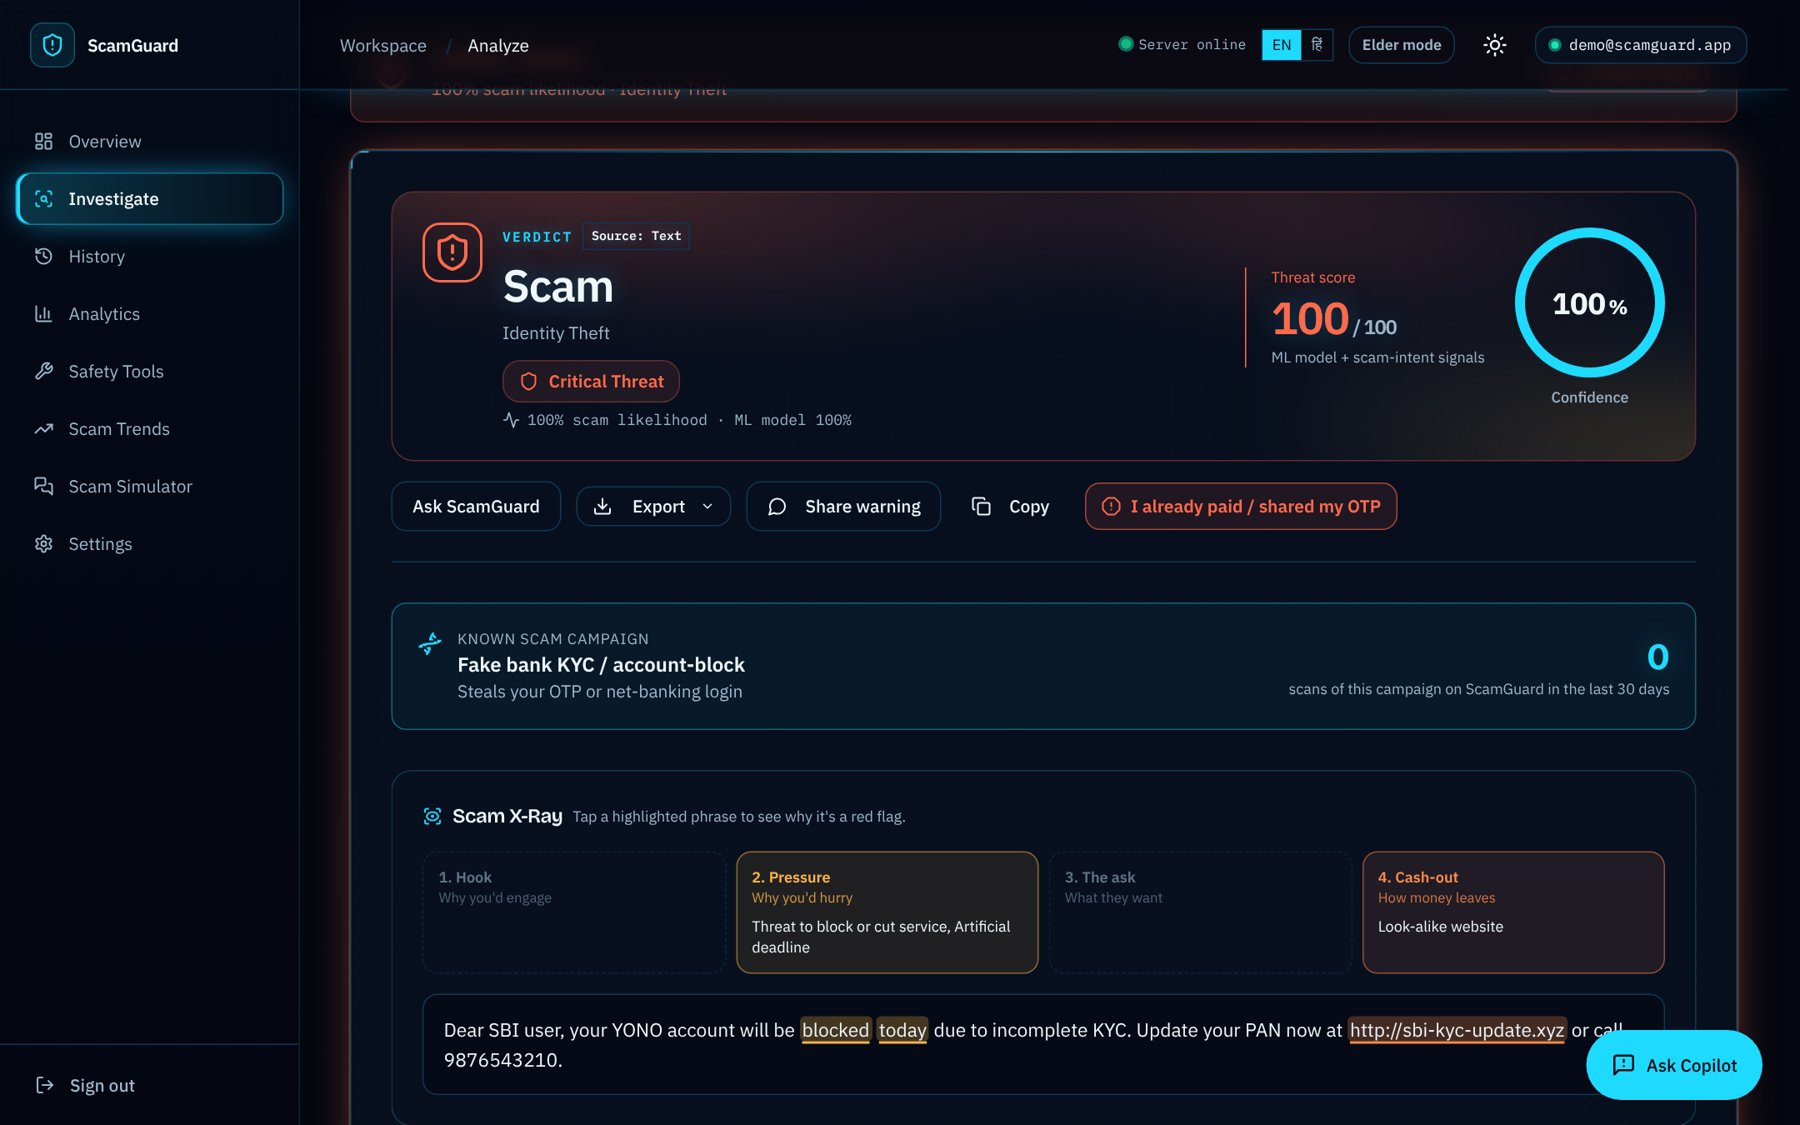
\includegraphics[width=0.80\linewidth,height=0.36\textheight,keepaspectratio]{shots/06_analyze_xray.jpg}}\caption{Scam X-Ray: each risky phrase placed in the hook, pressure, request and cash-out stages}\end{figure}
\begin{figure}[H]\centering\fbox{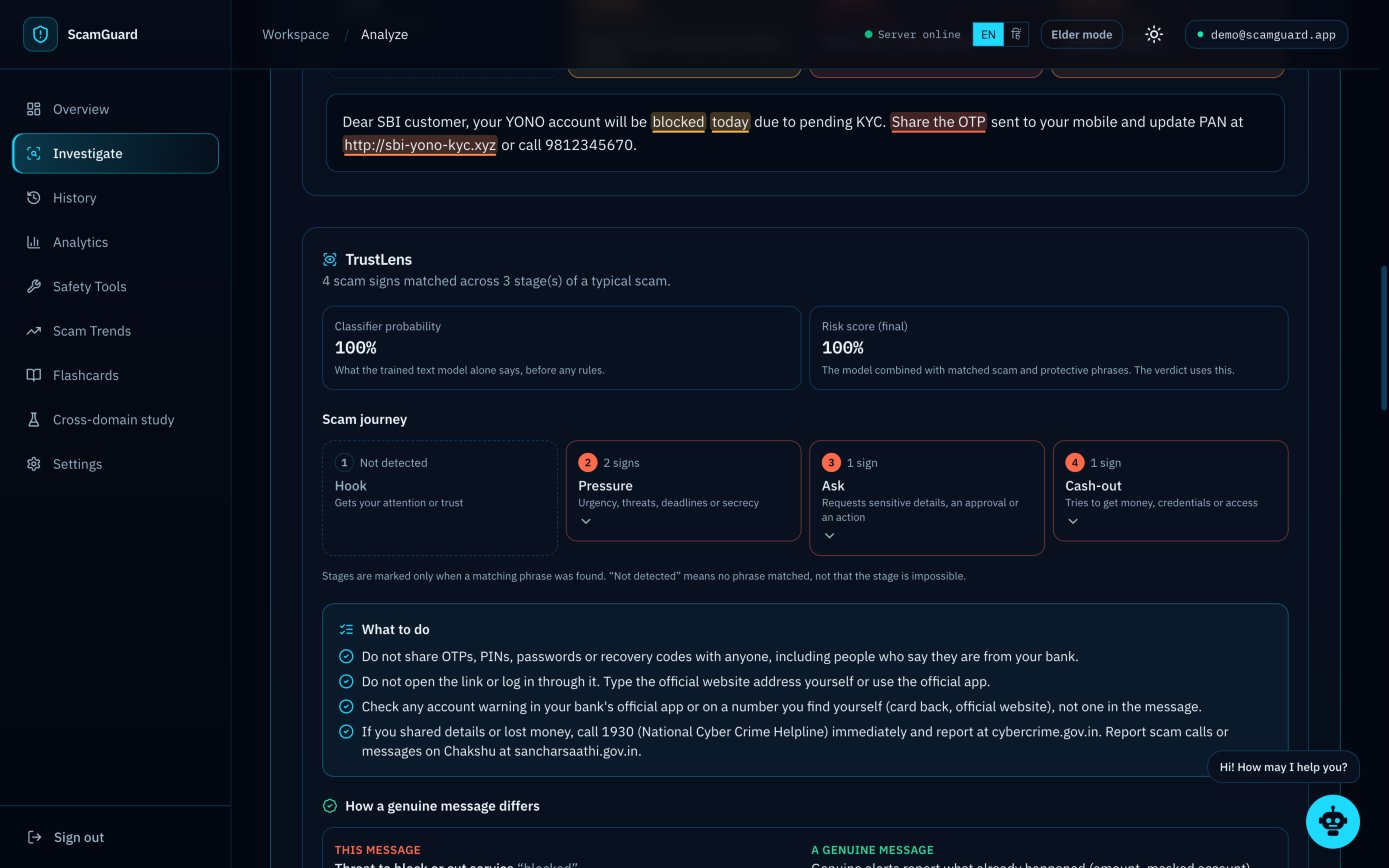
\includegraphics[width=0.80\linewidth,height=0.36\textheight,keepaspectratio]{shots/07_analyze_trustlens.jpg}}\caption{TrustLens: scam journey, recommended actions and how a genuine message differs}\end{figure}
\begin{figure}[H]\centering\fbox{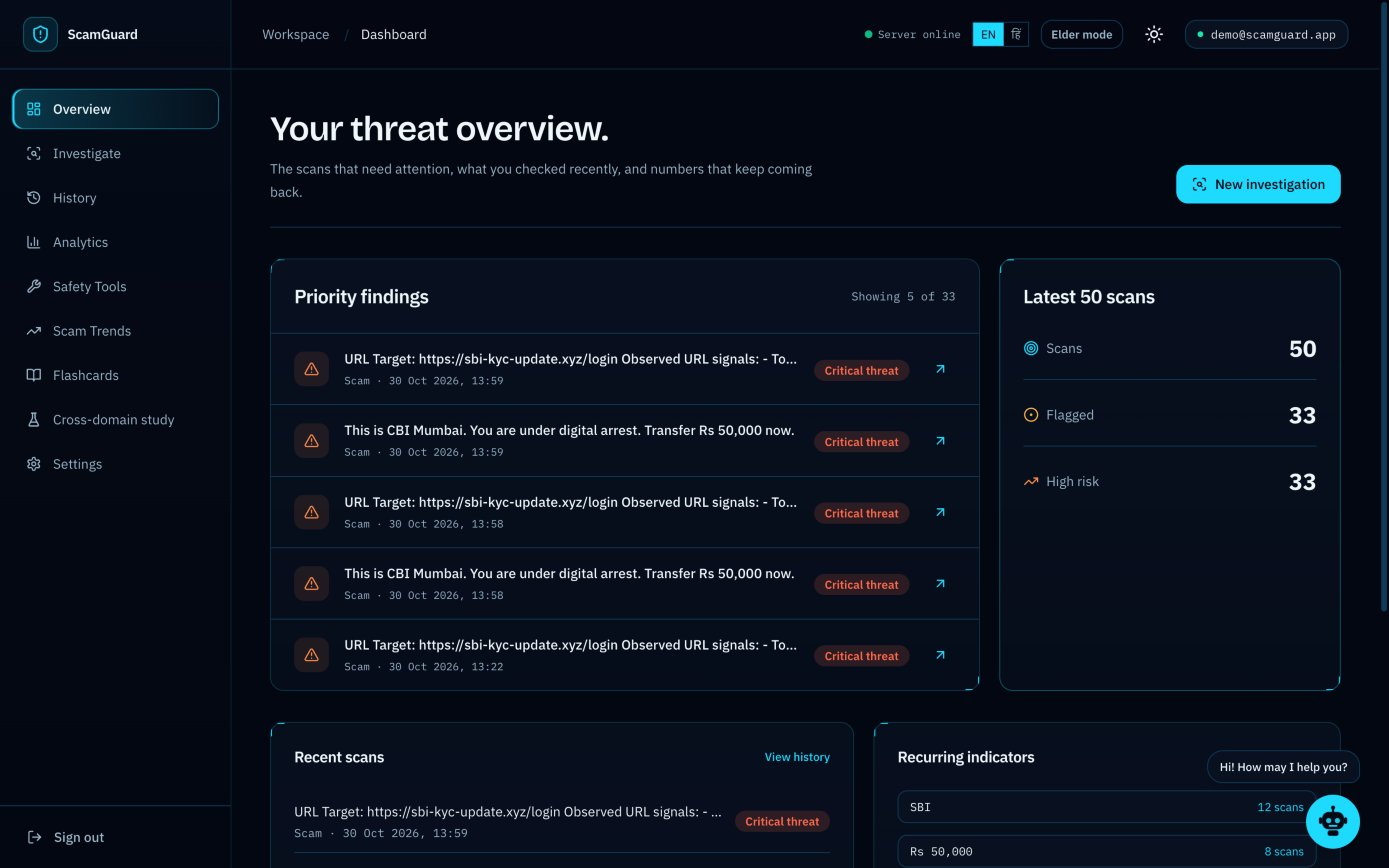
\includegraphics[width=0.80\linewidth,height=0.36\textheight,keepaspectratio]{shots/08_dashboard.jpg}}\caption{Dashboard with priority findings and recent scans}\end{figure}
\begin{figure}[H]\centering\fbox{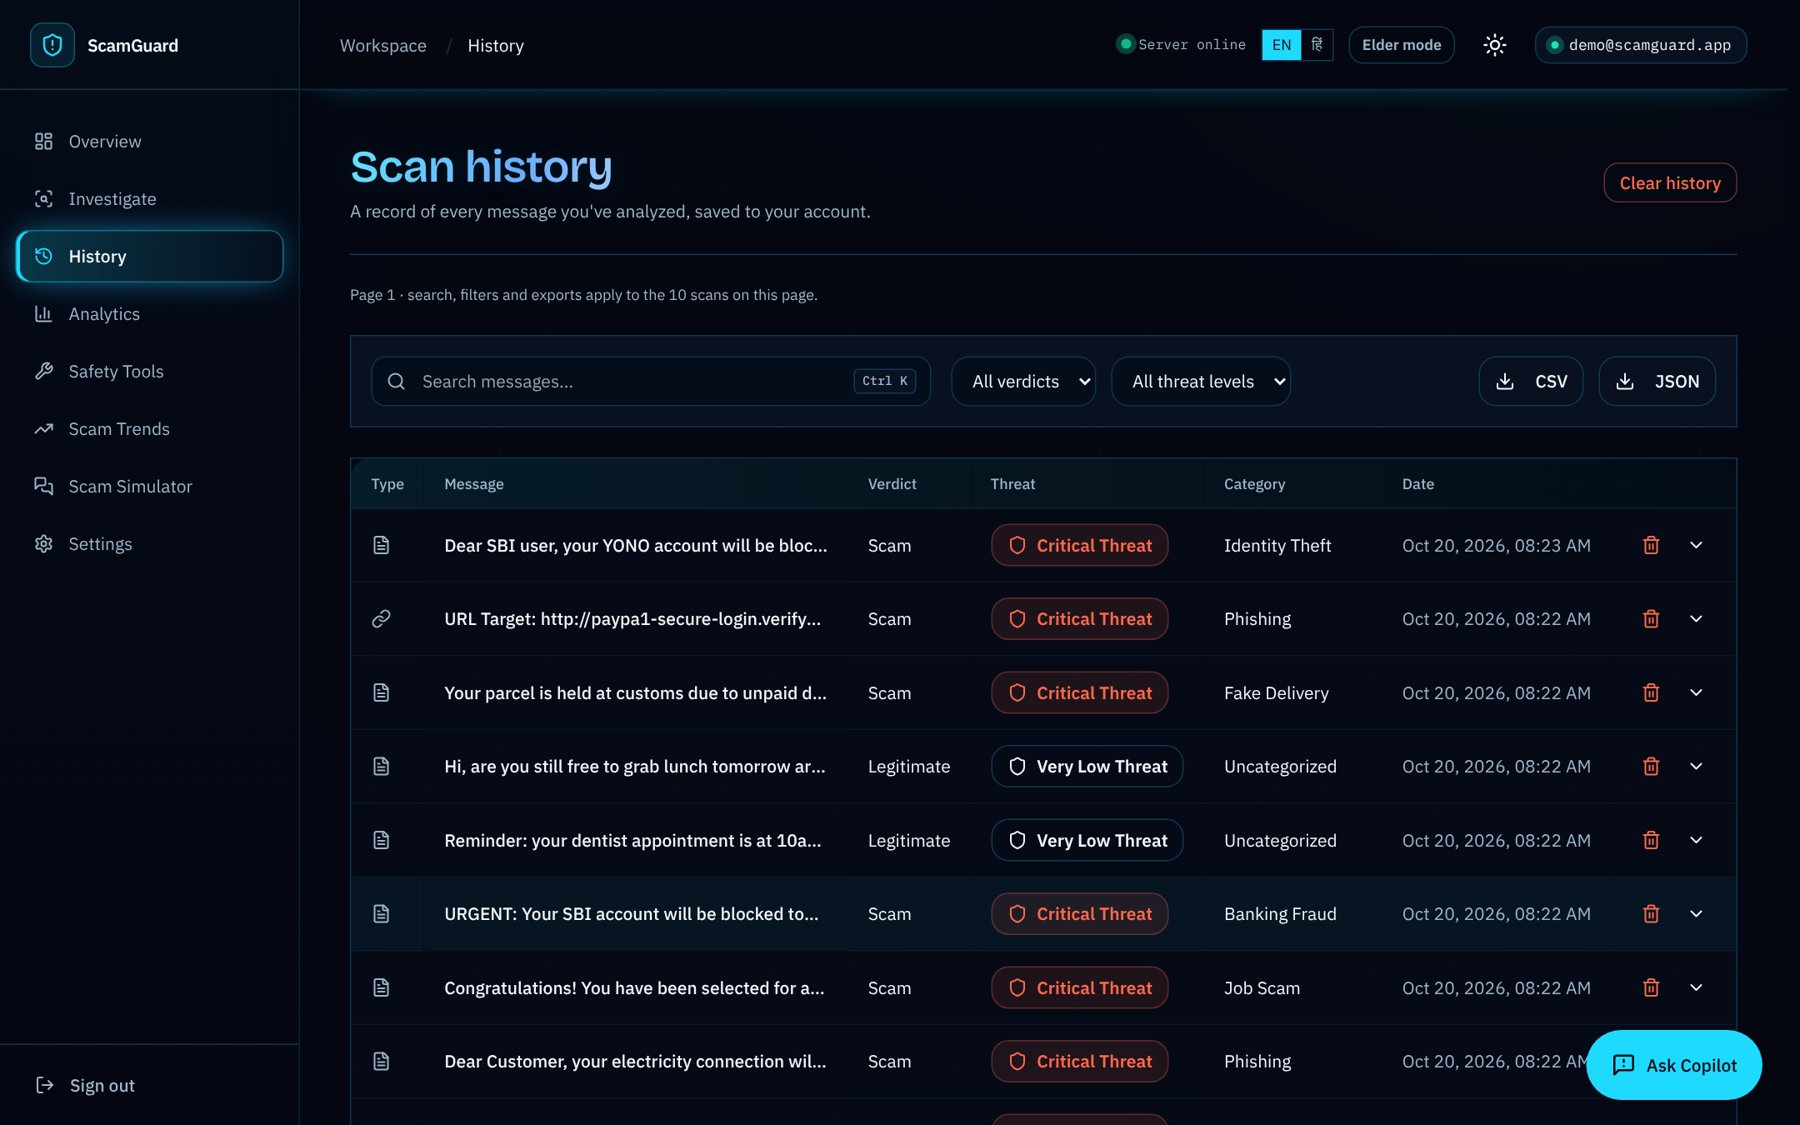
\includegraphics[width=0.80\linewidth,height=0.36\textheight,keepaspectratio]{shots/09_history.jpg}}\caption{Scan history with search, filters and export}\end{figure}
\begin{figure}[H]\centering\fbox{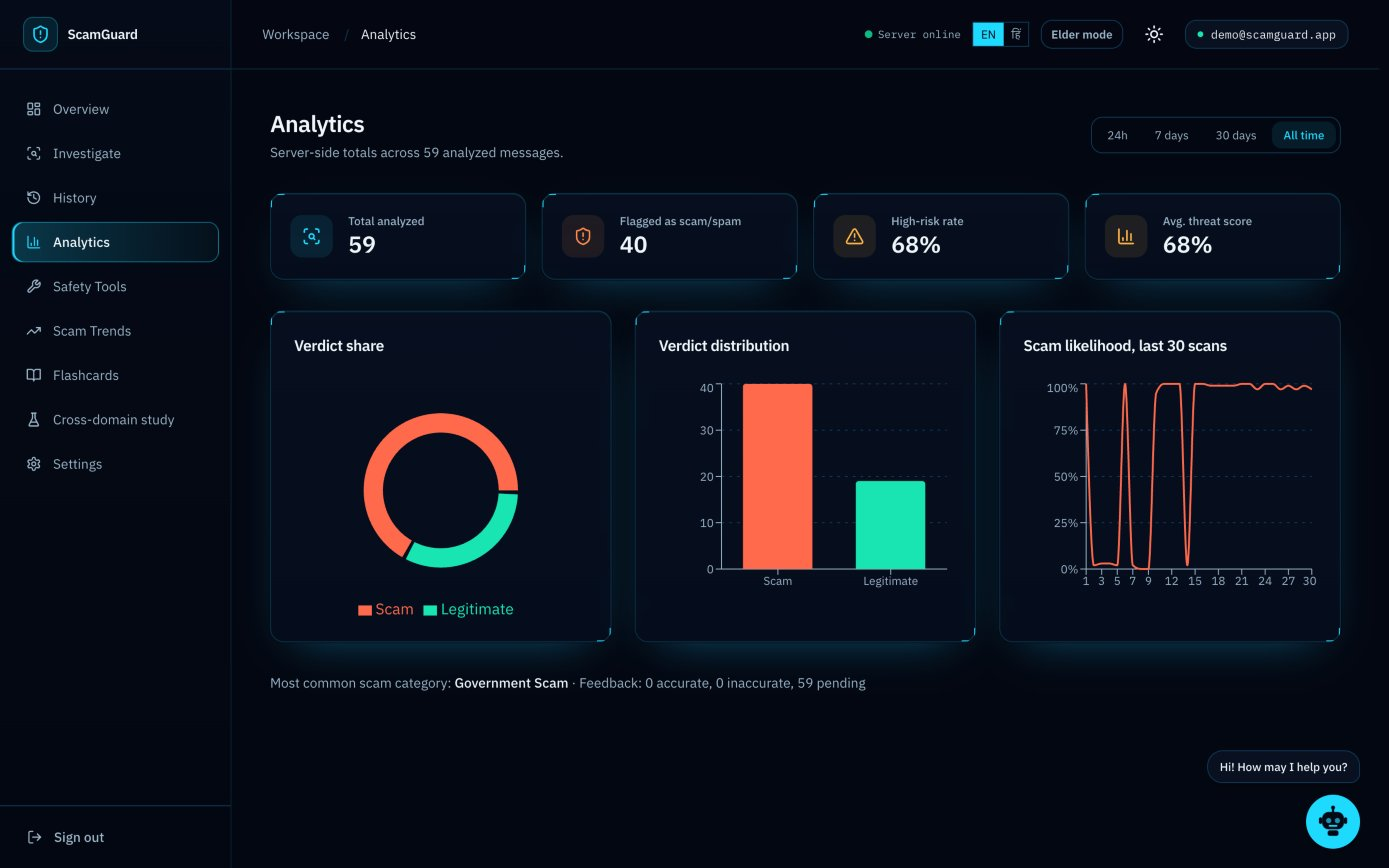
\includegraphics[width=0.80\linewidth,height=0.36\textheight,keepaspectratio]{shots/10_analytics.jpg}}\caption{Analytics: verdict share, distribution and score trend}\end{figure}
\begin{figure}[H]\centering\fbox{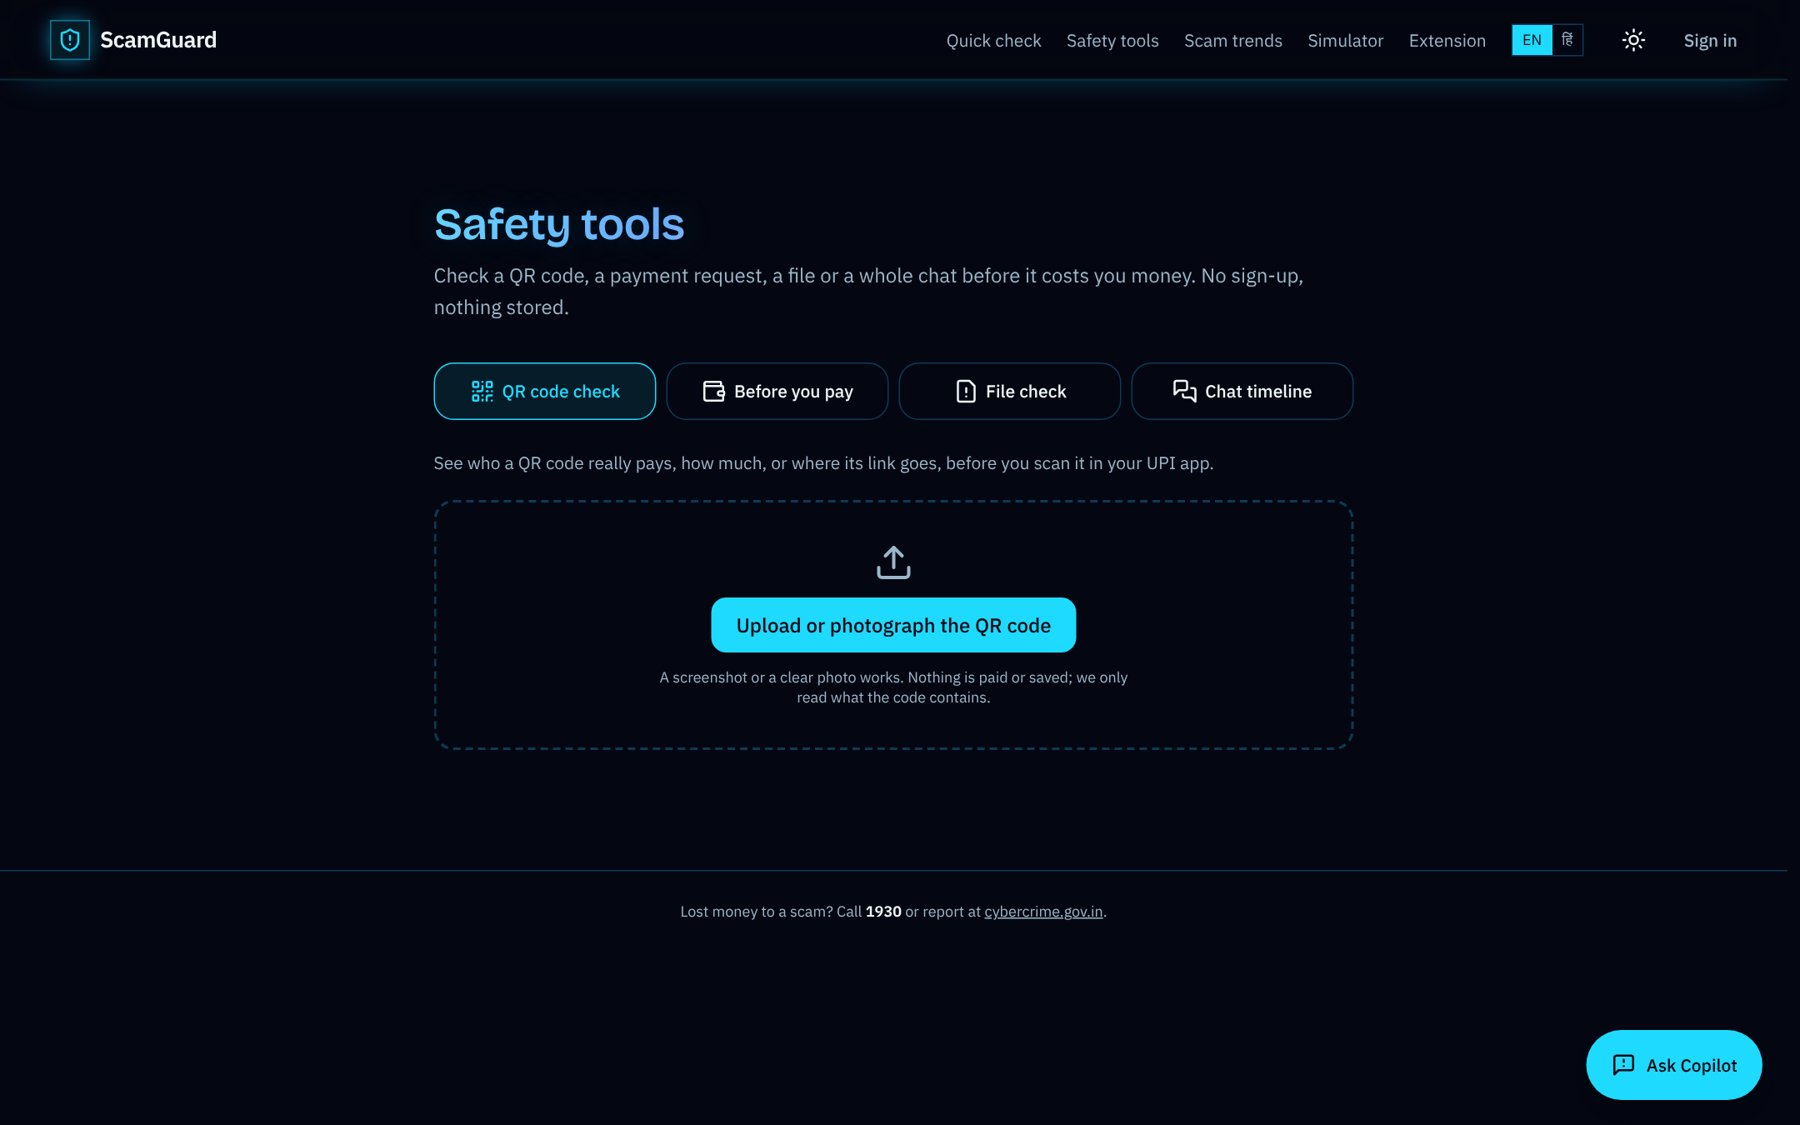
\includegraphics[width=0.80\linewidth,height=0.36\textheight,keepaspectratio]{shots/11_tools.jpg}}\caption{Safety tools: QR code check, before-you-pay, file check and chat timeline}\end{figure}
\begin{figure}[H]\centering\fbox{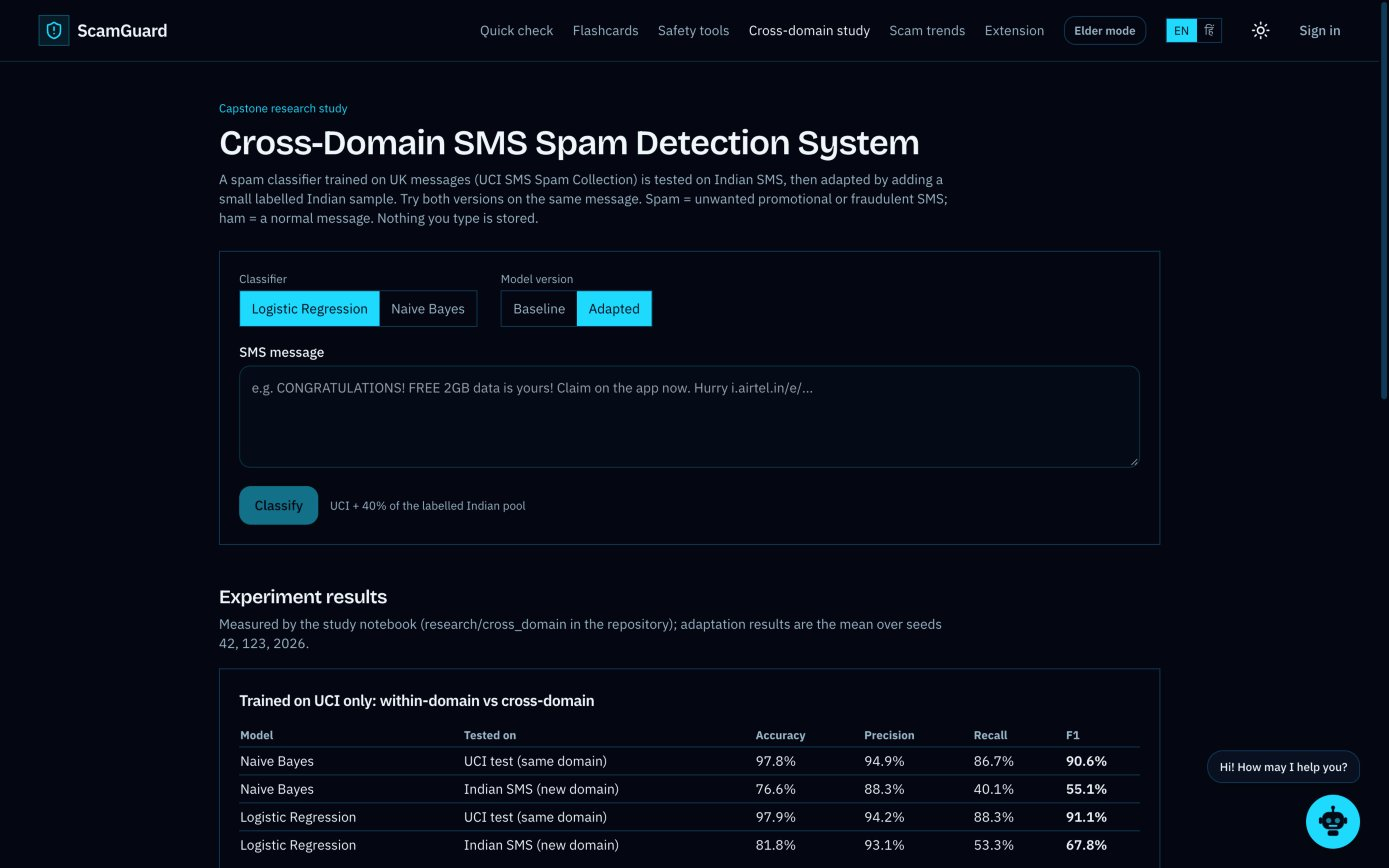
\includegraphics[width=0.80\linewidth,height=0.36\textheight,keepaspectratio]{shots/12_cross_domain.jpg}}\caption{Cross-domain page: the adapted model flags an Indian promotion that the baseline misses}\end{figure}

\appendixchapter{APPENDIX B: Details of list of publications related to this project}
Two manuscripts have been prepared from this project in the IEEE conference format. The first has been submitted for review; the second is yet to be submitted.

\vspace{0.3cm}\noindent\textbf{Paper 1}\\[4pt]
\begin{tabular}{@{}L{5.2cm}L{8.6cm}@{}}
Author Names: & Kayarvizhy N, Priyam Thakur, Bhavya Goyal, Samir Chaudhary, Sana Subodh \\[4pt]
Paper Title: & ScamGuard: AI-Based Online Scam and Fraud Detection System \\[4pt]
Name of the Conference or Journal: & 3rd International Conference on Computing for Sustainability and Intelligent Future (COMP-SIF 2027), Track 3: Cyber Resilience for Sustainability \\[4pt]
Status: & Submitted, under review \\[4pt]
Place of the Conference: & -- \\[4pt]
Date of Conference: & -- \\
\end{tabular}

\vspace{0.6cm}\noindent\textbf{Paper 2}\\[4pt]
\begin{tabular}{@{}L{5.2cm}L{8.6cm}@{}}
Author Names: & Kayarvizhy N, Priyam Thakur, Bhavya Goyal, Samir Chaudhary, Sana Subodh \\[4pt]
Paper Title: & Cross-Domain Generalization and Lightweight Domain Adaptation for SMS Spam Detection \\[4pt]
Name of the Conference or Journal: & To be decided (manuscript prepared in IEEE conference format) \\[4pt]
Place of the Conference: & -- \\[4pt]
Date of Conference: & -- \\
\end{tabular}

\appendixchapter{APPENDIX C: Details of Patent}
No patent has been filed or published for this project.

\appendixchapter{APPENDIX D: Details of Funding}
The project received no external funding. It was built with free cloud tiers and open-source software.

\appendixchapter{APPENDIX E: POs and PSOs Mapped}
\renewcommand{\thetable}{E.\arabic{table}}
\setcounter{table}{0}
Table~\ref{tab:po} maps the project to the eleven Programme Outcomes (POs) and gives the level at which each is addressed (1 = low, 2 = medium, 3 = high).

{\renewcommand{\arraystretch}{1.35}
\setstretch{1}\footnotesize\setlength{\tabcolsep}{5pt}
\begin{longtable}{|L{3.2cm}|>{\centering\arraybackslash}p{1.5cm}|L{9.4cm}|}
\caption{Programme Outcomes Mapping with ScamGuard and Domain Adaptation}\label{tab:po}\\
\hline
\textbf{PROGRAMME OUTCOMES} & \textbf{Level (1/2/3)} & \textbf{Justification if addressed} \\
\hline
\endfirsthead
\hline
\textbf{PROGRAMME OUTCOMES} & \textbf{Level (1/2/3)} & \textbf{Justification if addressed} \\
\hline
\endhead
PO1: Engineering Knowledge & 3 & Machine learning, NLP and statistics are used both to build the scam classifier and to judge how well it works. \\
\hline
PO2: Problem Analysis & 2 & We studied why current filters struggle with Indian SMS and traced the problem to unchecked labels, leaky evaluation and domain shift. \\
\hline
PO3: Design/Development of Solutions & 2 & A dataset, a detector and a web application were designed to meet targets for accuracy, speed and explanation. \\
\hline
PO4: Conduct Investigations of Complex Problems & 3 & Experiments are controlled: held-out campaigns, a separate target domain, bootstrap intervals, three seeds and significance tests. \\
\hline
PO5: Engineering Tool Usage & 3 & Modern tools throughout: scikit-learn, MinHash, FastAPI, Next.js, Streamlit, GitHub Actions and cloud hosting. \\
\hline
PO6: The Engineer and The World & 2 & Helps people avoid financial fraud and directs them to legal reporting channels (1930, cybercrime.gov.in). Runs on free, low-power servers with no GPU. \\
\hline
PO7: Ethics & 2 & Personal data is masked, dataset licences (CC BY 4.0, MIT) are followed and limitations are stated openly. The complete report was checked with DrillBit plagiarism detection software: 3\% similarity and 5.77\% AI-generated content (Appendix F), so the work is original and every source used is cited. \\
\hline
PO8: Individual and Collaborative Team work & 2.5 & Each of the four students owned one part (data, model, back end, front end) and the parts were joined into one working system. \\
\hline
PO9: Communication & 2 & Results reach readers through this report, two research papers, a presentation and an interface that explains each verdict. \\
\hline
PO10: Project Management and Finance & 2 & Work was planned in two phases; free-tier hosting and open-source tools kept the cost at zero. \\
\hline
PO11: Life-Long Learning & 2.5 & We learned MinHash, confident learning and domain adaptation on our own, and revised earlier claims when new data contradicted them. \\
\hline
\end{longtable}}


\appendixchapter{APPENDIX F: Similarity report, AI Generated report}
\renewcommand{\thefigure}{F.\arabic{figure}}
\setcounter{figure}{0}
\begin{figure}[H]\centering
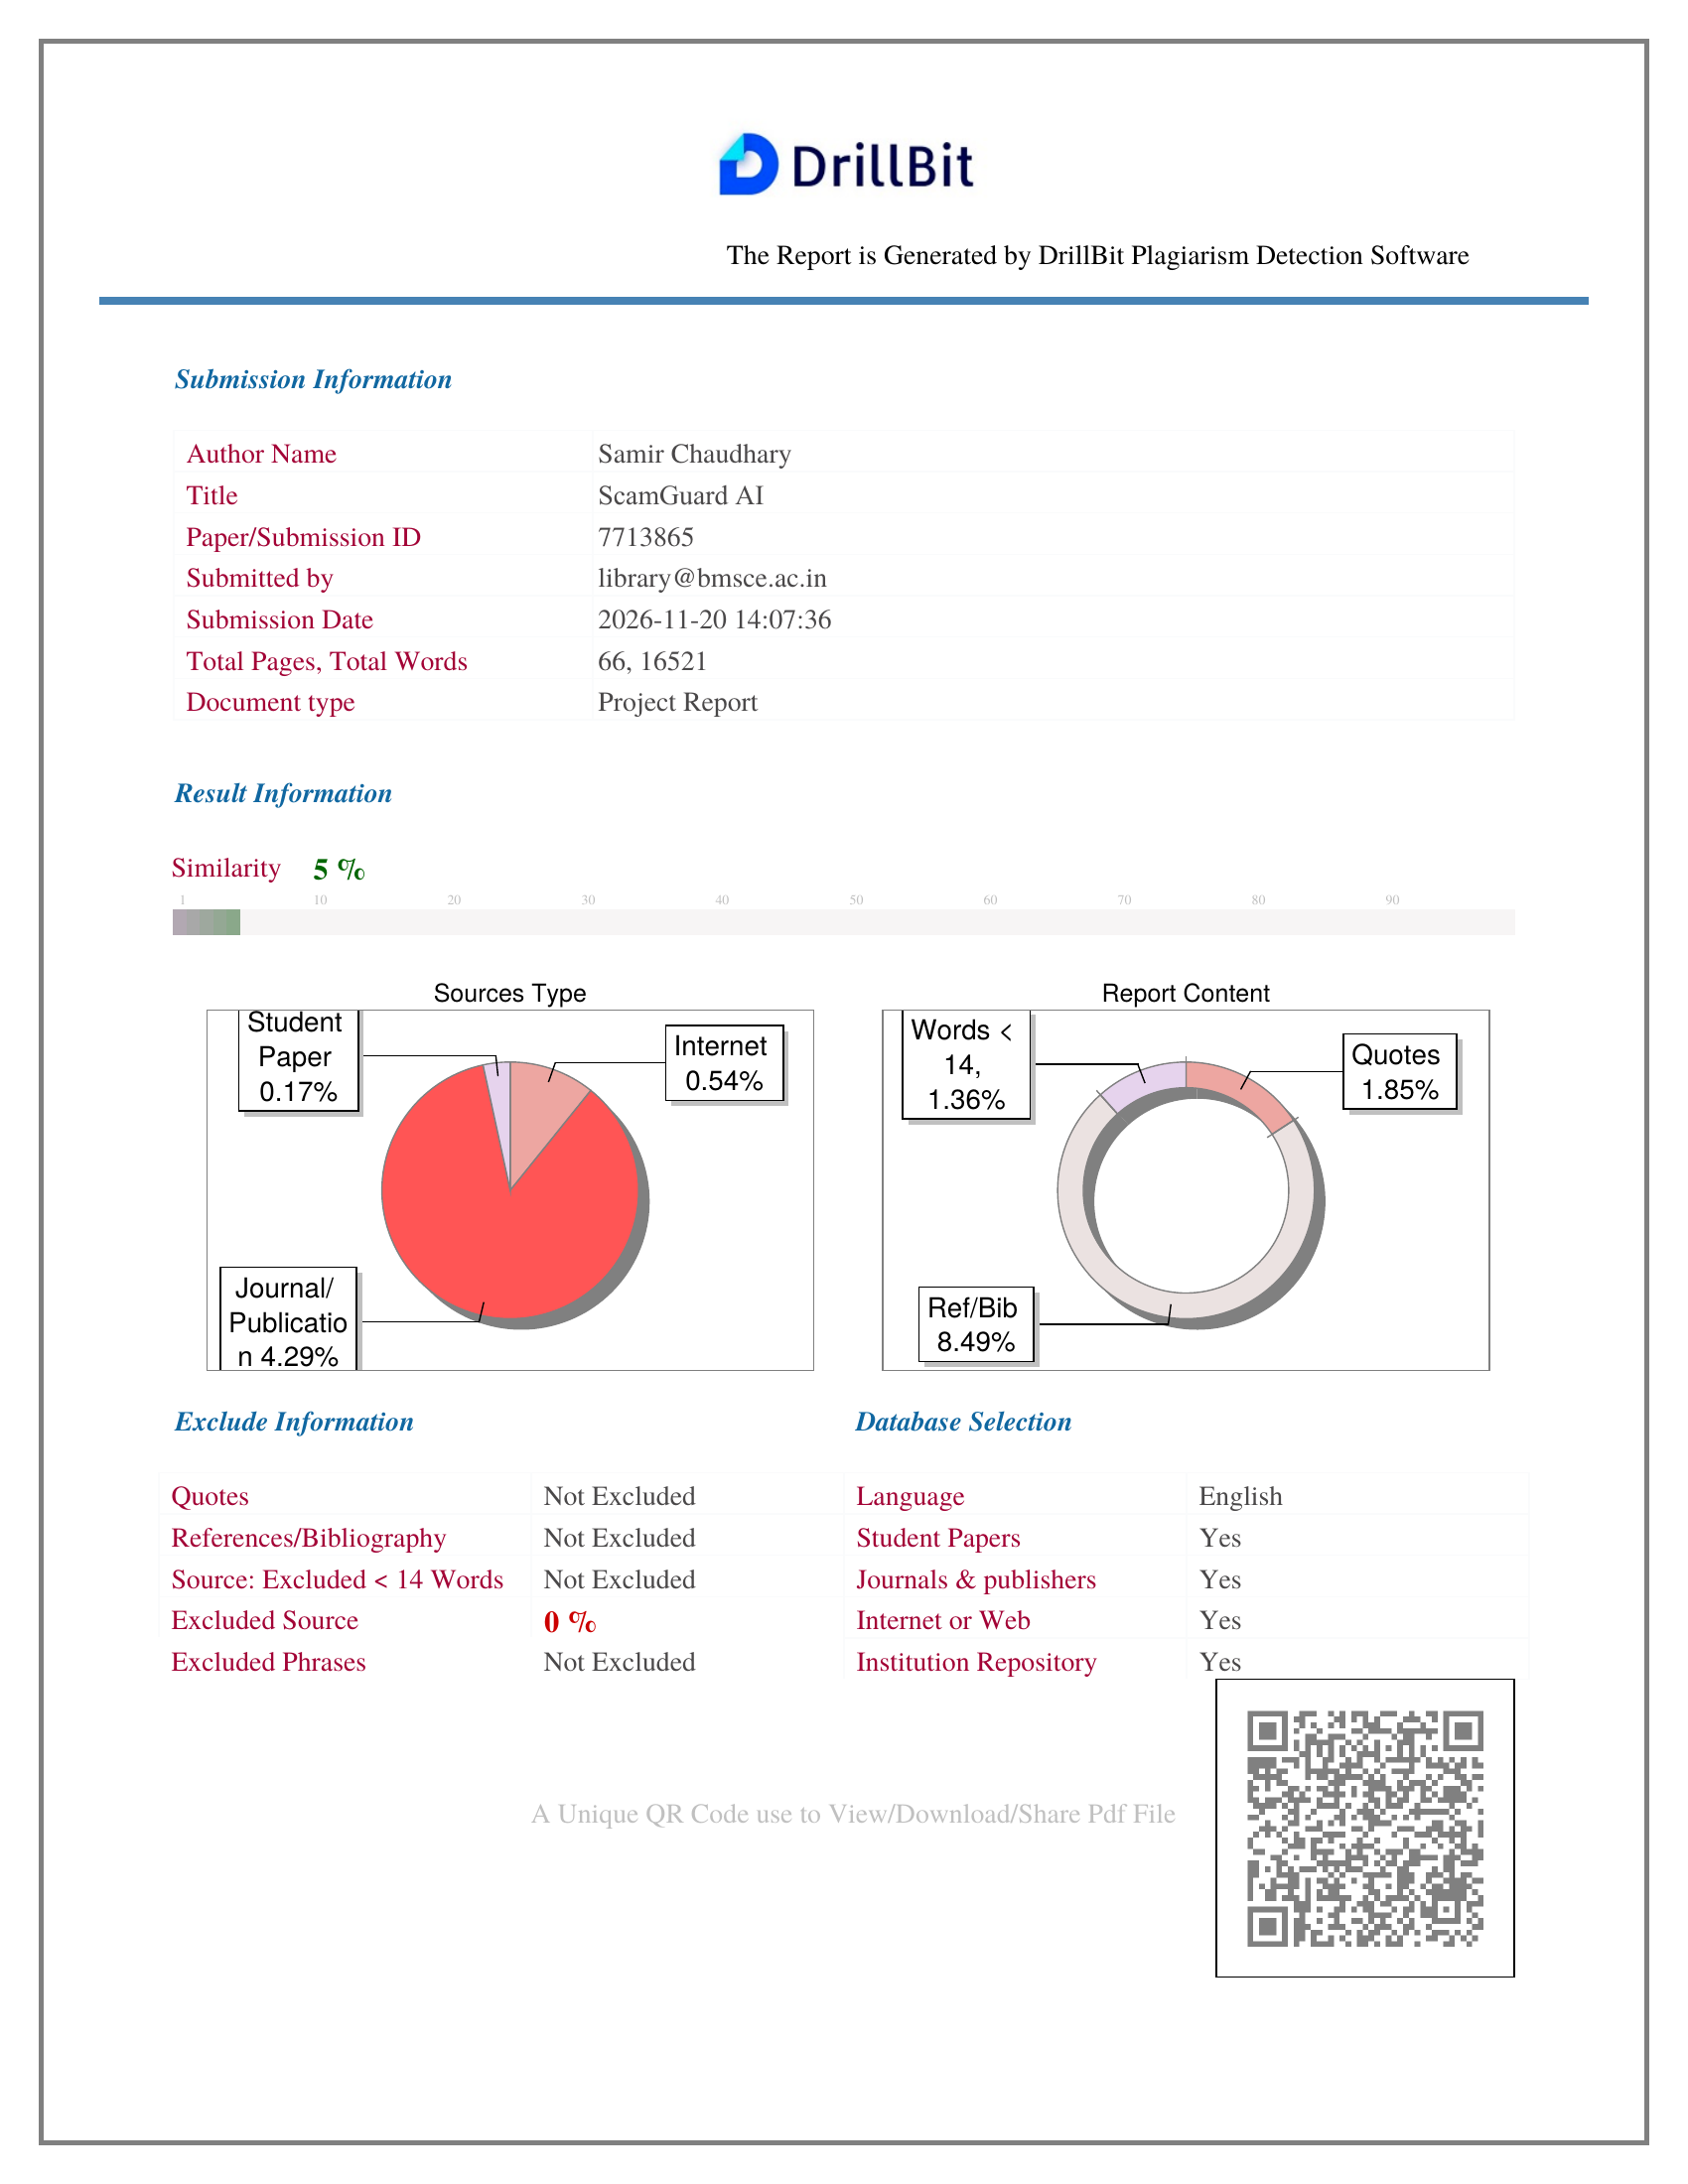
\includegraphics[width=\linewidth,height=0.78\textheight,keepaspectratio]{plag/similarity.png}
\caption{Similarity report (DrillBit plagiarism detection)}
\end{figure}
\clearpage
\begin{figure}[H]\centering
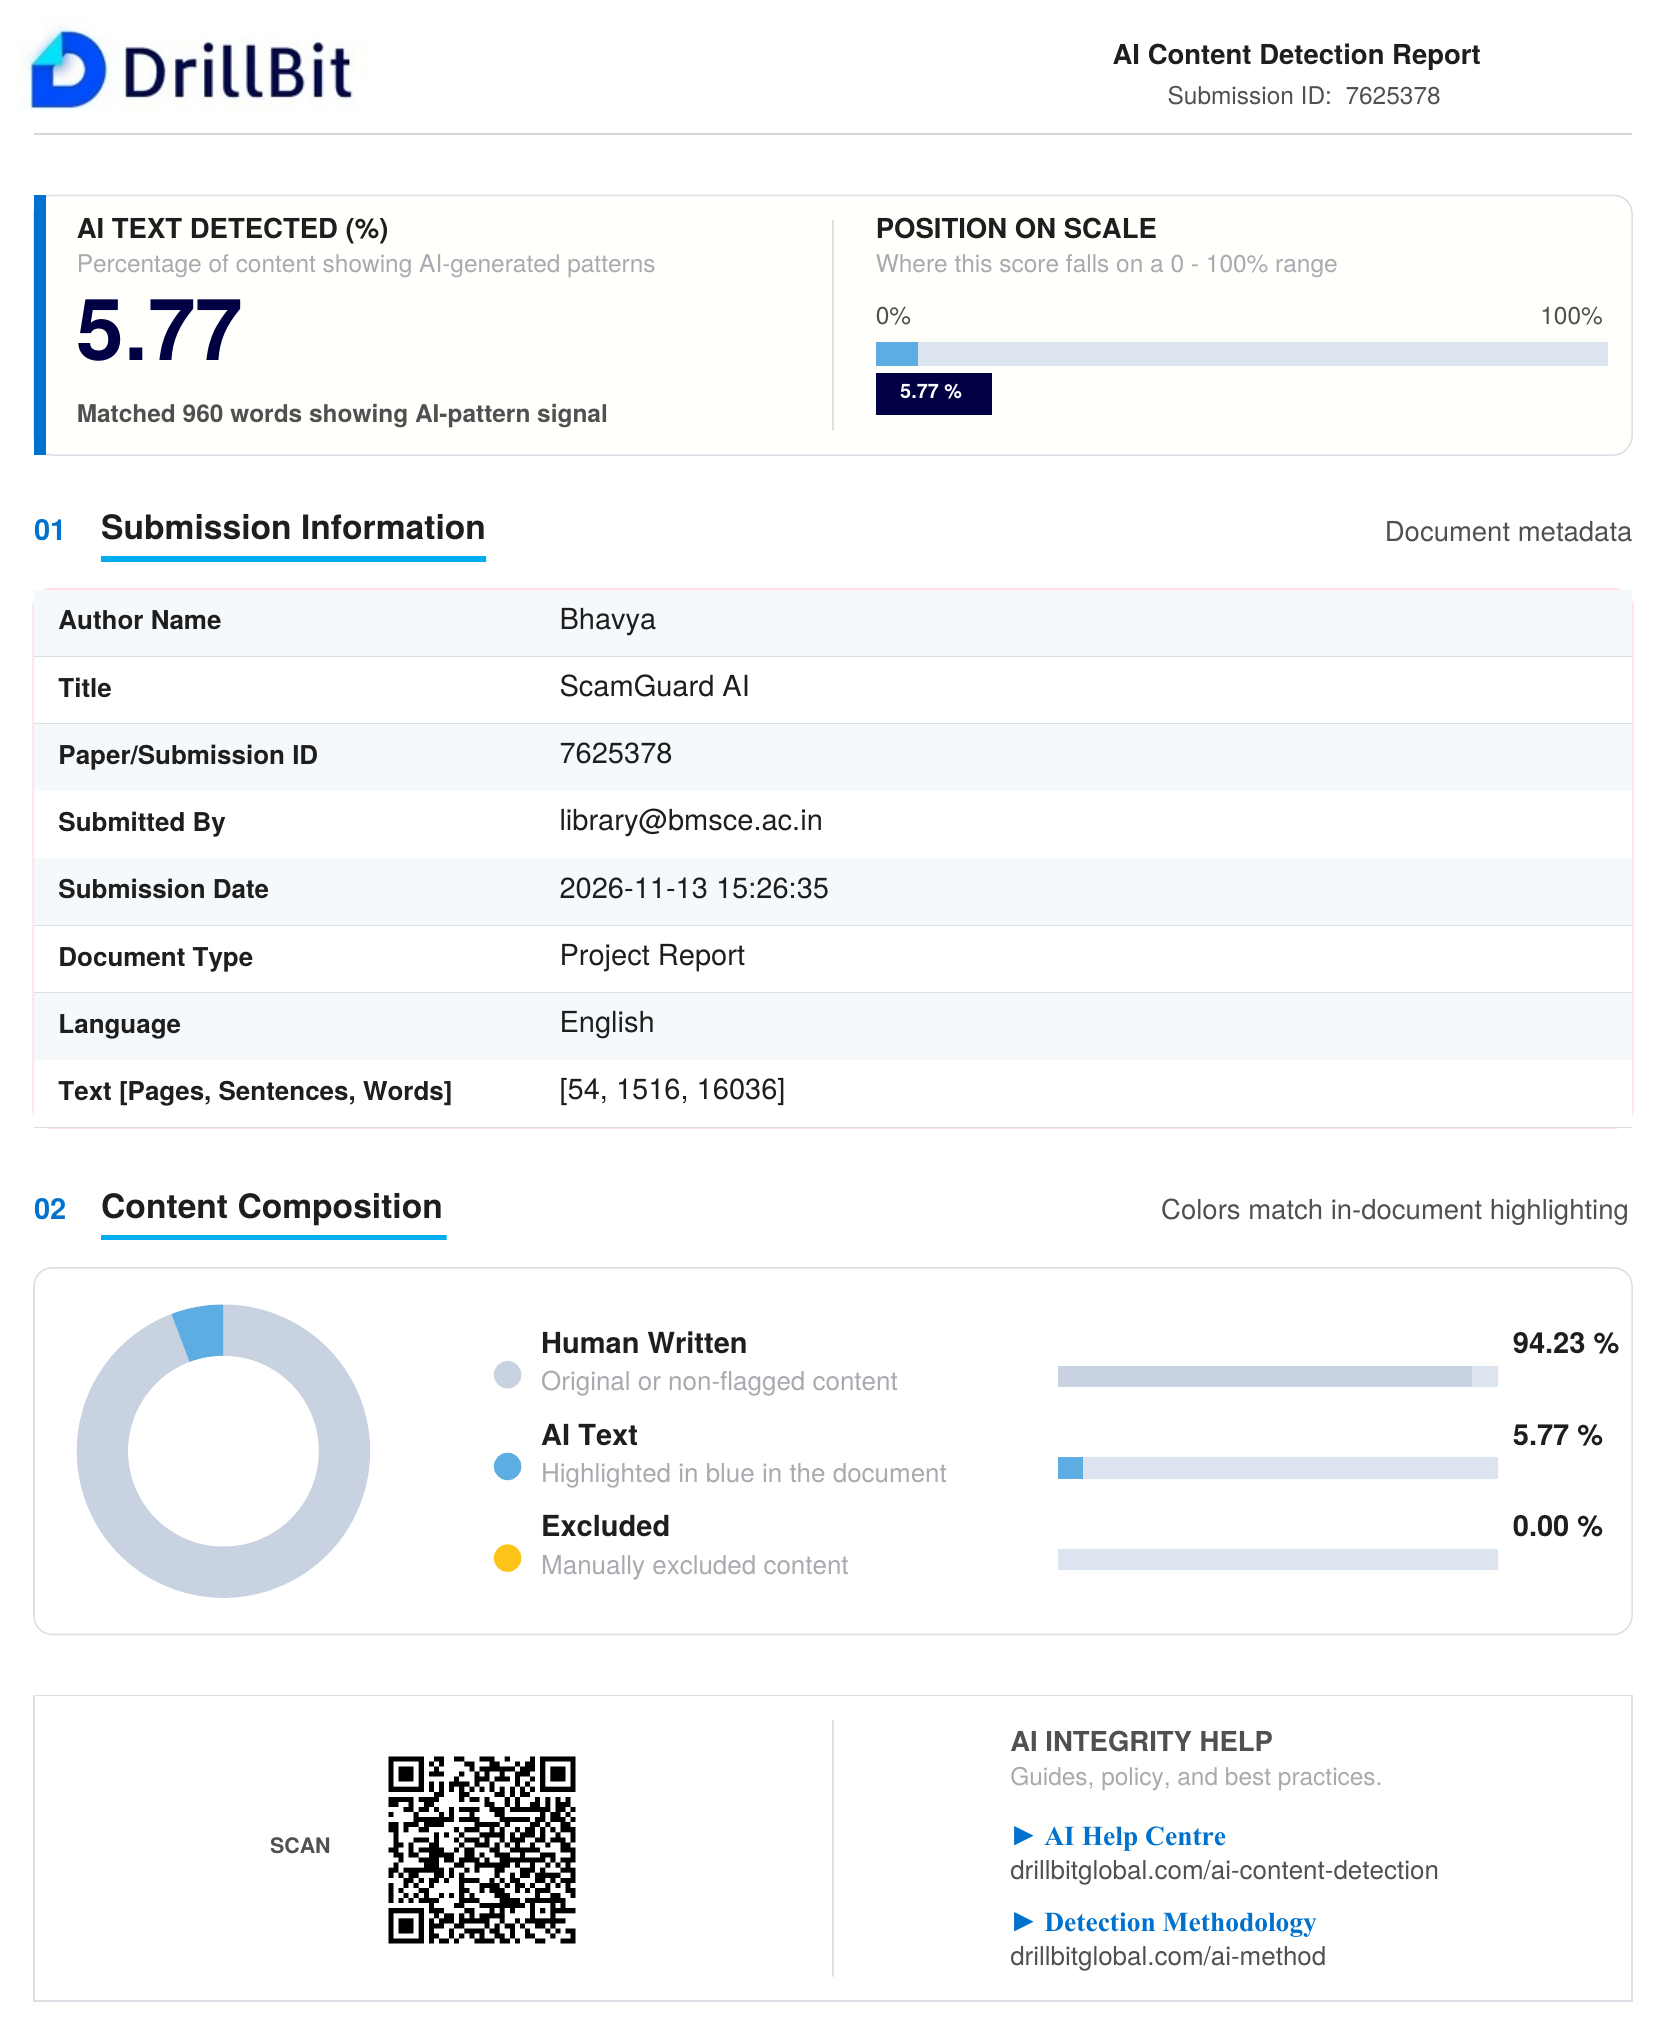
\includegraphics[width=\linewidth,height=0.80\textheight,keepaspectratio]{plag/ai_report.png}
\caption{AI-generated content report (DrillBit)}
\end{figure}
